\documentclass{article}
\usepackage{xeCJK}
\usepackage{listings} %插入代码
\usepackage{graphicx}
\usepackage{indentfirst}
\setCJKsansfont[BoldFont=STHeiti]{STXihei}
\setCJKmonofont{STFangsong}
\title{数据库专题训练大作业报告}
\author{赖国堃 2012011372}
\date{2016/10}
\begin{document}
\maketitle
\section{问题描述}
本次大作业问题为,从数据库中找出相似的路径,这里相似的定义是一条路径中的每个节点到另一条路径的距离均小于一个阈值,这里的距离代指欧几里得距离。\par
自然的对于这个问题,我们有两种看待的方式,一个是静态的,即假设已知所有的路线,我们的目标是找出所有的相似路线。另外一种是动态的,即系统主要处理对于一条询问路线,数据库中有多少条相似路线,并且数据库中可以动态的添加路线。接下来我们主要将问题设定为动态的并进行研究。
\section{算法设计}
\subsection{朴素}
最简单的方法就是对于每个询问路径,对于其中的每个节点,我们从数据集中的所有候选路径中找到在指定距离内的路径,缩小候选范围后,继续对下个节点进行检索。这个方法最简单,但是时间略慢。
\subsection{朴素优化}
首先,我们可以注意到由于数据是表示一条条路径,所以当前节点与上一节点在地理位置的概念上是比较接近的,那么我们可以知道,如果当前路径与另外一条路径相似,那么当前节点到另一条路径的最近点,应该在上一节点到另一条路径的最近点的附近。所以对于朴素算法中的候选路径,我们都记录上次是在哪个位置到上一节点的距离在阈值内,然后采用贪心的方法向前向后搜索。结果证明这个方法虽然简单,但是十分有效。
\subsection{R-tree优化}
经过上一个小节的优化后,我们发现我们找到最初的候选集还是比较低效的,最初我们是将所有的路径都作为候选路径,所以我们发现我们必然会遍历一便所有的路径。并且大部分路径是不相似的,这也就意味着我们一定要遍历一遍数据库中的所有节点。\par

这个是相当低效的,如果减少我们的遍历的量呢? 我们可以回到我们最初的问题,找到一个点距离在一个阈值之内的路径,路径可以被分解为线段,所以就等价为找到一个点距离在一个阈值之内的线段。由于是欧几里得距离,所以可以转化为,以一个节点为圆心,阈值为半径做圆,平面上那些线段与其相交或在其之内。\par

上面这个问题略为复杂,我们可以将其放松一下,我们知道一个线段与圆相交的必要条件是,这个线段的矩形需要与圆的外切正方形相交,如下图所示。\par
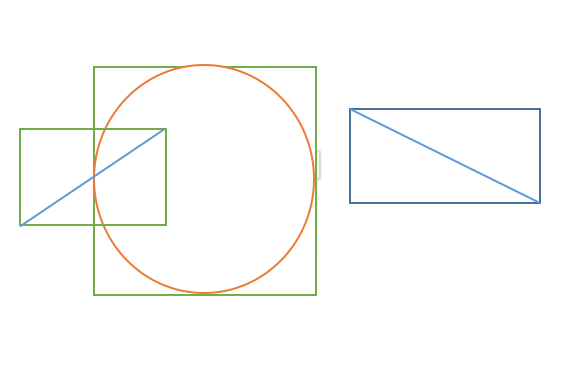
\includegraphics{example.png}

这样我们就可以用R-tree来维护这个二维矩形集合,并且快速访问。由于大作业中数据全部给出,为了实现方便,所以我们采用R-tree简化版kd-tree,他们实现原理类似,只是kd-tree不支持插入节点,所有数据必须在初始化时候给出,但是两者实际的效果是相似的。\par

\subsection{进一步优化}

我们注意到我们可以利用R-tree来减小我们的候选集合,对于一条路径,起始点,我们肯定需要用R-tree来决定我们的候选集合,但是下一个节点,由于其距离起始点距离较近,所以我们采用朴素方法会取得更好的效果(由于朴素的检索范围为候选集合,而R-tree为全体路径集合)。但是我们希望一个更小的其实候选集合,由数据是出租车数据,我们可知,起点和终点的差异应该较大,自然的,我们可以对起点进行R-tree筛选,然后再对终点进行筛选,这样我们能够进一步减小候选集合。

\section{文件列表}

pusu.cpp 朴素算法。\par

main.cpp 结合kd-tree的算法。\par

kd-tree.cpp kd-tree.h kdtree的实现文件。\par

common.h common.cpp 模型中使用的数据结构以及通用函数(如经纬度距离转化函数)。\par

\section{实验结果}

\section{可采用的优化}

对于算法设计的最后一个小节,我认为从一个路径当中多选取几个点,利用R-tree所有候选集合是一个进一步提高效率的策略,但是我们需要注意,R-tree和朴素应该是一个平衡的关系,我们需要细致的实验和大量数据的验证来找到一个比较好的平衡点。
\end{document}
